\section{Results}

\subsection{Predictions from the infinite-horizon model}

I first analyze the findings from the infinite-horizon model on three fronts, the optimal portfolio share of the risky-asset for high-wealth individuals, the shape of the optimal portfolio share as a function of normalized monetary resources, and the effect of covariances between the income and asset shocks on the consumption function.

\subsubsection{Optimal portfolio share at high-wealth levels}

I start by looking at the baseline model with uncorrelated shocks to income and asset returns. Let the equity premium be set at 3 percent for this part of the analysis, and the standard deviation of the log shock to the equity return be set at 15 percent, i.e. $\s_{\nu} = 0.15$. Let all other parameters be as in Table \ref{tab:model_parameters}. Figure \ref{fig:baseline_portfolio} shows that the optimal portfolio allocation $\k(m)$ is 1 at low values of $m$ and decreases to an asymptotic value as $m$ tends to infinity.

\begin{figure}[h]
    \centering
    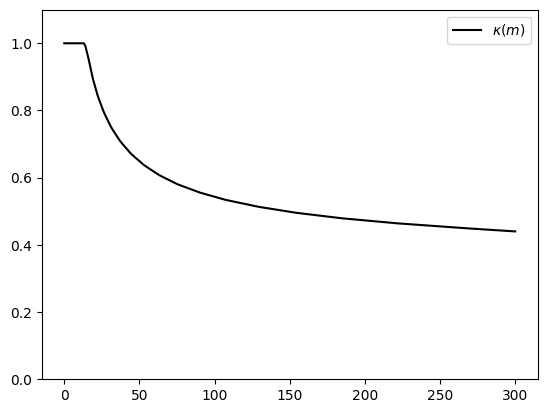
\includegraphics[width=0.6\textwidth]{kFunc_baseline.png}
    \caption{Optimal portfolio share with uncorrelated shocks}
    \label{fig:baseline_portfolio}
\end{figure}

It is well understood that this asymptotic value of $\k$ is positively related to the equity premium and negatively related to $\s_{\nu}$ [ADD GRAPHS IN APPENDIX]. The natural question, then, is the effect of a positive covariance between income shocks and asset returns on optimal asymptotic portfolio share.

\begin{figure}[h]
    \centering
    \begin{subfigure}{0.49\textwidth}
        \centering
        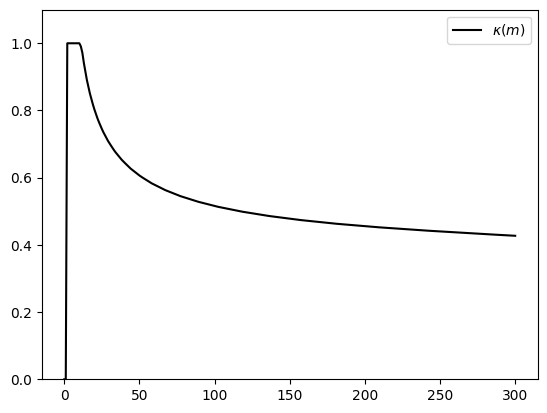
\includegraphics[width=0.8\textwidth]{kFunc_baseline_corrTransFull.png}
        \caption{Transitory shock ($\o_{\nu,\,\z} = 0.025$)}
        \label{subfig:correlated_baseline_transitory}
    \end{subfigure}
    \begin{subfigure}{0.49\textwidth}
        \centering
        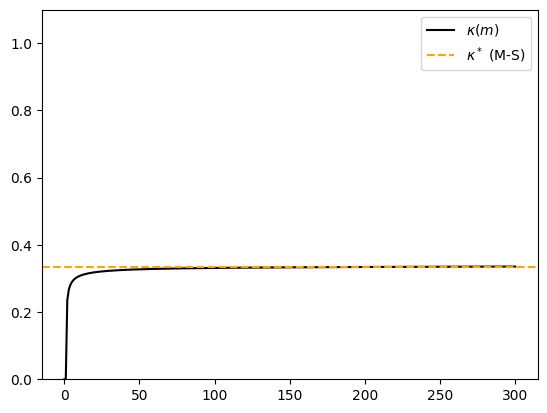
\includegraphics[width=0.8\textwidth]{kFunc_baseline_corr.png}
        \caption{Permanent shock ($\o_{\eta,\,\nu} = 0.008$)}
        \label{subfig:correlated_baseline_permanent}
    \end{subfigure}
    \caption{Optimal portfolio share under high correlation ($> 0.8$) between income shocks and asset returns}
    \label{fig:correlated_shock_baseline}
\end{figure}

Figure \ref{fig:correlated_shock_baseline} shows how optimal portfolio share responds to a correlation of greater than 0.8 between one of the income shocks and asset returns. Figure \ref{subfig:correlated_baseline_transitory} depicts the case when the transitory shock is correlated with asset returns. Since the optimal portfolio allocation is unaffected for all but the lowest values of $m$ (see section \ref{portfolio_low_wealth}), the asymptotic level of $\k$ remains the same as in the model with uncorrelated shocks. However, as Figure \ref{subfig:correlated_baseline_permanent} depicts, even with a completely different optimal portfolio allocation rule, for high levels of wealth, the optimal portfolio share tends to similar values as in the case with no correlations.

The explanation for this behavior can be found by examining the optimal portfolio share condition, given by:
\[
\E_{t}\bs{(\Rfree_{t+1} - \Rfix)(\Gc_{t+1}c(m_{t+1}))^{-\rho}} = 0
\]
where
\[
m_{t+1} = \frac{\Rc_{t+1}}{\Gc_{t+1}}(m_{t} - c_{t}) + \z_{t+1}
\]
Unquestionably, the covariances between the shocks affect the realized values of $m_{t+1}$, and therefore the realizations of future consumption given by $c(m_{t+1})$. However, for high values of $m_{t}$, given the nature of the consumption function and the low MPC out of wealth (see section \ref{consumption_baseline}), the variability of the amounts consumed in the future is fairly low. Moreover, consider levels of wealth sufficiently high such that $c(m)$ is large. Naturally, $c_{t+1}^{-\rho}$ is bound to be an extremely small quantity, implying that optimal values of $\k$ are likely to grow increasingly similar under the models with and without correlations in shocks as $m$ grows larger.

\subsubsection{Optimal portfolio share at low wealth}\label{portfolio_low_wealth}

While optimal portfolio shares at large wealth levels are not affected much by the correlation between shocks, we can observe a stark change in the share of the risky asset among individuals whose wealths are less than twice of their permanent incomes.

\begin{figure}[h]
    \centering
    \begin{subfigure}{0.49\textwidth}
        \centering
        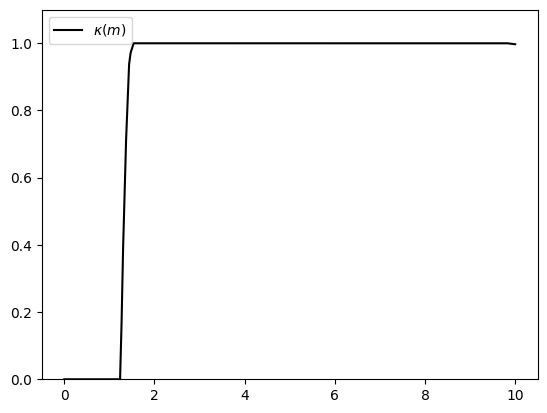
\includegraphics[width=0.8\textwidth]{kFunc_baseline_corrTrans.png}
        \caption{Transitory shock}
        \label{subfig:correlated_poor_transitory}        
    \end{subfigure}
    \begin{subfigure}{0.49\textwidth}
        \centering
        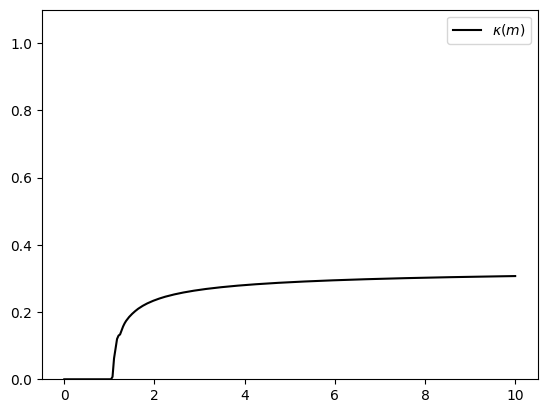
\includegraphics[width=0.8\textwidth]{kFunc_baseline_corrZoomed.png}
        \caption{Permanent shock}
        \label{subfig:correlated_poor_permanent}
    \end{subfigure}
    \caption{Individuals with low wealth invest all their savings in the risk-free asset}
    \label{fig:baseline_correlated_poor}
\end{figure}

Figure \ref{fig:baseline_correlated_poor} shows that agents with normalized wealth less than 2 (somewhere between 1 and 2 to be precise), invest all their savings in the risk-free asset, irrespective of whether asset returns are correlated with transitory or permanent income shocks. At low levels of savings, notice that $\z_{t+1}$ comprises the major component of $m_{t+1}$, and high covariance between $\nu_{t+1}$ and $\z_{t+1}$ implies that low values of $\z_{t+1}$ go with low values of $\nu_{t+1}$. Since the marginal utility of future consumption is high at low values of $m_{t+1}$, which coincides with low values of $\Rfree_{t+1}$, greater weight is placed on instances with low asset returns when taking the expectations in equation (\ref{eq:excess_return}). This lowers the optimal portfolio share of the risky asset, in this case to 0. The other situation is when $\nu$ is correlated with $\eta$. Given the equation of $m_{t+1}$, this actually reduces the variability in $c(m_{t+1})$. However, the positive correlation between $\nu$ and $\eta$ implies that when $\Rfree_{t+1} - \Rfix$ is negative, $\Gc_{t+1}$ is low, implying that $\Gc_{t+1}^{-\rho}$ is higher. Thus, the instances of negative return are weighted higher in the excess return equation. Supposing that $\nu$ and $\eta$ are perfectly correlated, if $\k  1$, then $m_{t+1} - \z_{t+1}$ becomes a constant, and the higher weight accorded to instances with negative return implies that the expectation becomes negative. On the other hand, if $\k = 0$, negative values of $\Rfree_{t+1} - \Rfix$ are coupled with low values of $\Gc_{t+1}$ and therefore higher $m_{t+1}$, implying that the lower marginal utility of normalized consumption under negative excess returns makes $\k = 0$ closer to optimality.

The second aspect is how the optimal portfolio share looks for slightly higher levels of wealth. Upto $m \approx 1.5$, agents consume almost all of their monetary resources and save next to nothing (see section \ref{consumption_baseline}). As such, the high MPC out of consumption causes variability in future monetary resources to translate into variability in future consumption at an almost one-to-one level. After a certain threshold, however, the MPC sharply falls, and the concavity of the consumption function ensures that it continues to fall. Moreover, due to the diminishing marginal utility of consumption and the very low magnitude of the marginal-marginal-utility of consumption, variability in $m_{t+1}$ translates to very little variability in $c(m_{t+1})^{-\rho}$. The analysis of the finite horizon model in section \ref{finite_horizon} shows that the marginal utility channel accounts for most of this effect as opposed to the MPC.

In that light, see that the argument for why optimal $\k$ is low when permanent income shocks and returns are correlated does not crucially depend on the value of $a_{t+1}$ being extremely low, and the optimal $\k$ is always lower than the asymptotic value. However, when looking at the case with correlation between $\z$ and $\nu$, note that the only channel through which there is any effect is the marginal utility of consumption, or $c(m_{t+1})^{-\rho}$. By the discussion above, this has less of an effect at higher values of $m_{t+1}$, and the optimal portfolio allocation rule resembles the one in the model with uncorrelated shocks.

\subsubsection{Optimal consumption policy}\label{consumption_baseline}

While the properties of the consumption function in the buffer stock model are well understood, I reiterate some important features to augment that arguments provided above. Figure \ref{fig:baseline_consumption} shows the optimal consumption function.

\begin{figure}[h]
    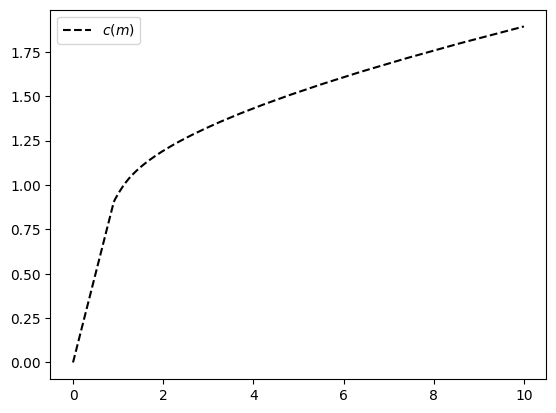
\includegraphics[width=0.6\textwidth]{cFunc_baseline_zoomed.png}
    \caption{Optimal consumption function in the buffer-stock model}
    \label{fig:baseline_consumption}
\end{figure}

Under the artificial no-borrowing constraint, the $c(m) \leq m$, which implies that $c$ is both defined only for $m \geq 0$ and has a kink at the point where the borrowing constraint begins to bind. For this region, the MPC is 1, implying that for low values of $m$, as remarked earlier, the total  savings rate is extremely low. However, the MPC sharply falls beyond this point. Appendix [ADD ONE] shows that the optimal consumption policy in the models with correlated shocks remains mostly unchanged. The low MPC for high values of $m$ thus leads to the ineffectiveness of transitory shocks in affecting optimal portfolio choice.

\subsection{Next-to-last period in finite-horizon}\label{finite_horizon}

Due to the convergence properties of the consumption function, we know that the optimal consumption rule in the finite-horizon model for periods sufficiently away from the last period closely approximate the infinite horizon consumption rule. As such, if the next period's consumption is similar to the infinite-horizon consumption, the optimal portfolio allocation rule should also be similar to the infinite-horizon rule. On the other end of this discussion is the period that is next to last.

The consumer in the last period knows that their optimization problem in the last period boils down to maximizing utility from current-period consumption, which implies that $c_T(m_T) = m_T$. The first useful feature of this is that it provides us with a consumption function for which we have an analytical expression, which allows us to rewrite the optimal portfolio allocation condition as:
\[
\E_{T-1}\bs{(\Rfree_{T} - \Rfix)(\Rc_{T}a_{T} + \Gc_{T}\z_{T})^{-\rho}}
\]
While the coincidence of negative values of $\Rfree_{T} - \Rfix$ and small values of $\Gc_{T}$ still holds true, the MPC out of total monetary resources is a constant 1. As a result, the only channel through which the portfolio choice problem differs at high $m_{T-1}$ as opposed to low is the marginal utility of consumption. Figure [ADD APPENDIX] shows that the optimal portfolio allocation is nearly identical to that in the infinite horizon problem, showing that the low MPC implied by the consumption function in the infinite-horizon problem plays a negligible role in affecting the portfolio choice of the wealthy.

\subsection{Calibrating to U.S. Data}

While the previous sections distil the primary insights from the model with an artificial parameterization of asset returns, both in terms of the equity premium and the variability of the returns from equity, I now look at how the model responds to being calibrated to parameters documented in the literature about U.S. data. Since the primary determinant of optimal portfolio allocation in the model that is of interest to us is the correlation between permanent income shocks and shocks to the return on the risky asset, I vary this parameter while holding the others constant at documented values. To begin, \citet{Mehra1985} estimate that the historical real rate of return on equity in the U.S. is 7.67 percent, while the return on a relatively risk-free securities over the same period was 1.31 percent.\footnote{The original data was later updated till 2005, which forms the source of these estimates. See \citet{Mehra2006} for details.} Furthermore, the Sharpe ratio for these assets was calculated to be 0.37. Since $\nu$ is a mean-one lognormal, we know that:
\[
\s_{\nu}^2 = \log\bp{\bp{\frac{\Rfree - \Rfix}{0.37\Rfree}}^2 + 1}
\]
I follow \citet{Carroll2015} and set $\s_{\eta}^2 = \frac{0.04}{11}$ and $\s_{\z}^2 = 0.04$. Data on per capita income in the U.S. reveals that real income grew at an average rate of 2.16 percent. I also set $\b = 0.93$ and $\o_{\z,\,\eta} = \o_{\z,\,\nu} = 0$. I then solve the model using a baseline of $\rho = 4$ for different values of $\o_{\eta,\,\nu}$. The full choice of parameters is then given in Table \ref{tab:model_parameters}.

\begin{table}[htbp]
    \begin{tabular}{ccc}
        \toprule
        Parameter & Value & Source\\
        \midrule
        $\rho$ & 4\\
        $\b$ & 0.93\\
        $\G$ & 1.0216 & \href{https://united-states.reaproject.org/analysis/comparative-indicators/growth_by_decade/per_capita_personal_income/reports/}{U.S. Data}\\
        $\Rfree$ & 1.0767 & \citet{Mehra2006}\\
        $\Rfix$ & 1.0131 & \citet{Mehra2006}\\
        $\s_{\nu}^2$ & 0.011 & \citet{Mehra2006}\\
        $\s_{\eta}^2$ & $0.01 \times \frac{4}{11}$ & \citet{Carroll2015}\\
        $\s_{\z}^2$ & 0.04 & \citet{Carroll2015}\\
        \bottomrule
    \end{tabular}
    \caption{Parameters used to solve the model}
    \label{tab:model_parameters}
\end{table}

\subsubsection{Preliminary findings}

The first thing we can see under this new parameterization is that even with highly collinear shocks ($\text{corr}(\log\nu,\,\log\eta) \approx 1$), the optimal portfolio share is 1. This is because despite the high covariance, the excess return of more than 6 percent and the relatively low volatility, with a standard deviation of under 10.5 percent for the logged shock to returns, makes it difficult to justify holding the risk-free asset. In fact, Figure \ref{fig:US_rho_comparison} shows that the equity share of portfolio falls to realistic levels only when $\rho$ is as large as 12. This number is close to the benchmark by \citet{Schreindorfer2020}, whose model incorporates disappointment averse preferences and has agents exhibit levels of relative risk aversion of close to 10.

\begin{figure}[h]
    \centering
    \begin{subfigure}{0.49\textwidth}
        \centering
        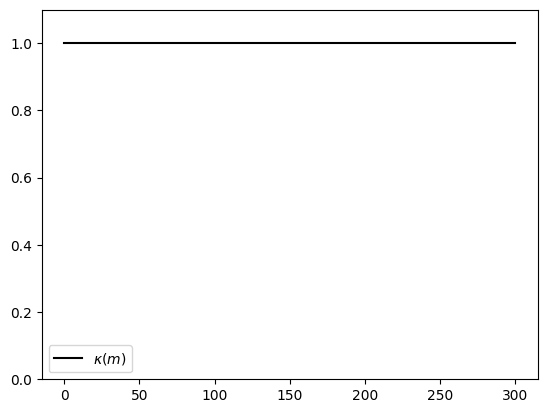
\includegraphics[width=0.8\textwidth]{kFunc_US_rho4.png}
        \caption{$\rho = 4$}
    \end{subfigure}
    \begin{subfigure}{0.49\textwidth}
        \centering
        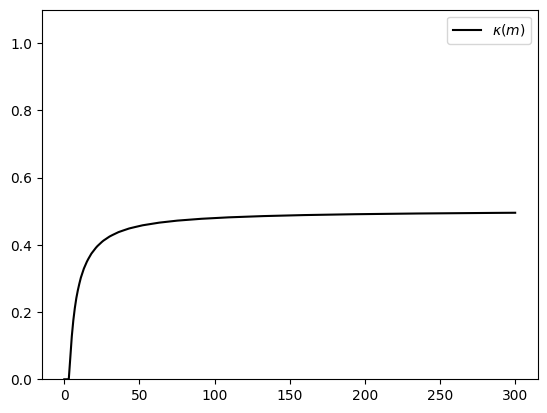
\includegraphics[width=0.8\textwidth]{kFunc_US_rho12.png}
        \caption{$\rho = 12$}
    \end{subfigure}
    \caption{U.S. figures requires extremely high CRRA to explain the equity premium}
    \label{fig:US_rho_comparison}
\end{figure}

One of the key issues with the 